\chapter{Image~Annotation}
\label{chap:annotation} 

This chapter describes the design, implementation of a human in the loop object detection system and details it's use annotating real datasets.

\section{Introduction}

\section {User interface}


\section {Implementation}

\begin{figure}[h]
  \centering
  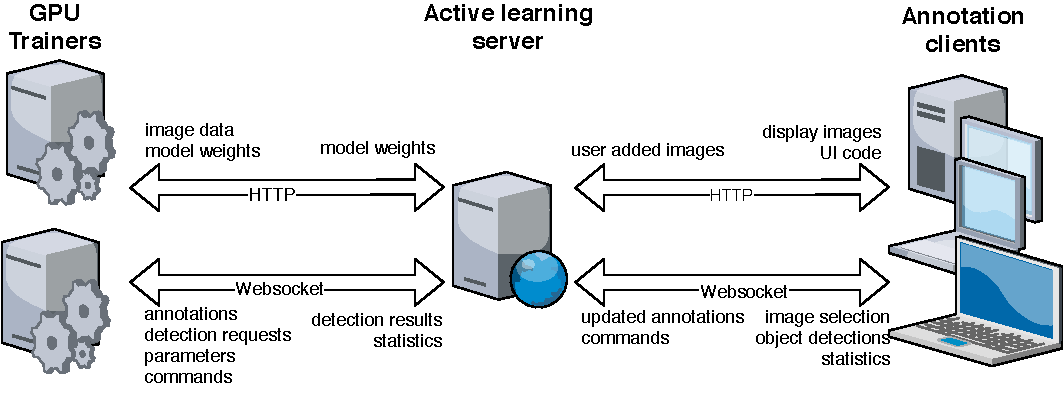
\includegraphics[width=0.9\linewidth]{annotation/data_flow.pdf}
  \caption{Data flow between services for the annotation system}  
  \label{fig:data_flow}
\end{figure}


\begin{figure}[h]
  \centering
  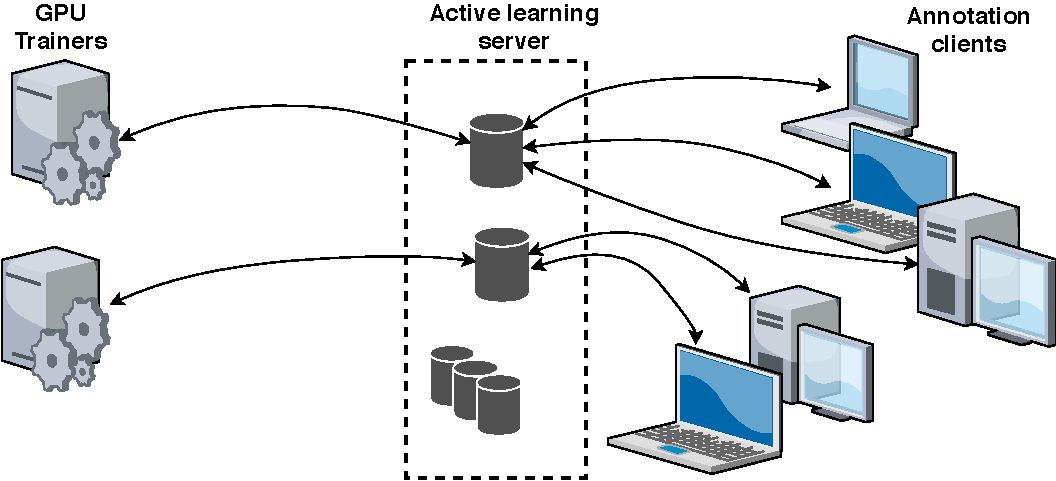
\includegraphics[width=0.9\linewidth]{annotation/connectivity.pdf}
  \caption{Connectivity of the annotation system}  
  \label{fig:connectivity}
\end{figure}

\section{Annotation studies}

\subsection {Penguins}
\subsection{Tree branch intersections}
\subsection{Scallop}


\section{Counting}

\subsection{Adelie Penguins}
\subsection{Waddell Seals}




\section {Reviewing mistakes}